\documentclass[11pt]{article}
\usepackage{graphicx}
\usepackage{array}
\usepackage{xcolor}
\usepackage[a4paper,total={8in,10in}]{geometry}
\usepackage{mdframed}
\usepackage{geometry}
\usepackage{hyperref}
\begin{document}
\begin{mdframed}[backgroundcolor=orange]
~
\begin{center}
\begin{Huge}
\color{white}{\fontfamily{pbk}\selectfont SIDDHANT}\color{gray}{\fontfamily{pbk}\selectfont\textbf{ BHAMBRI}}
\end{Huge}
\end{center}
\begin{center}
\begin{large}
\color{white}\emph{Aiming to use technology to bring a considerable positive change for mankind}
\end{large}
\end{center}
\end{mdframed}
\begin{minipage}{1.00\linewidth}
\begin{center}
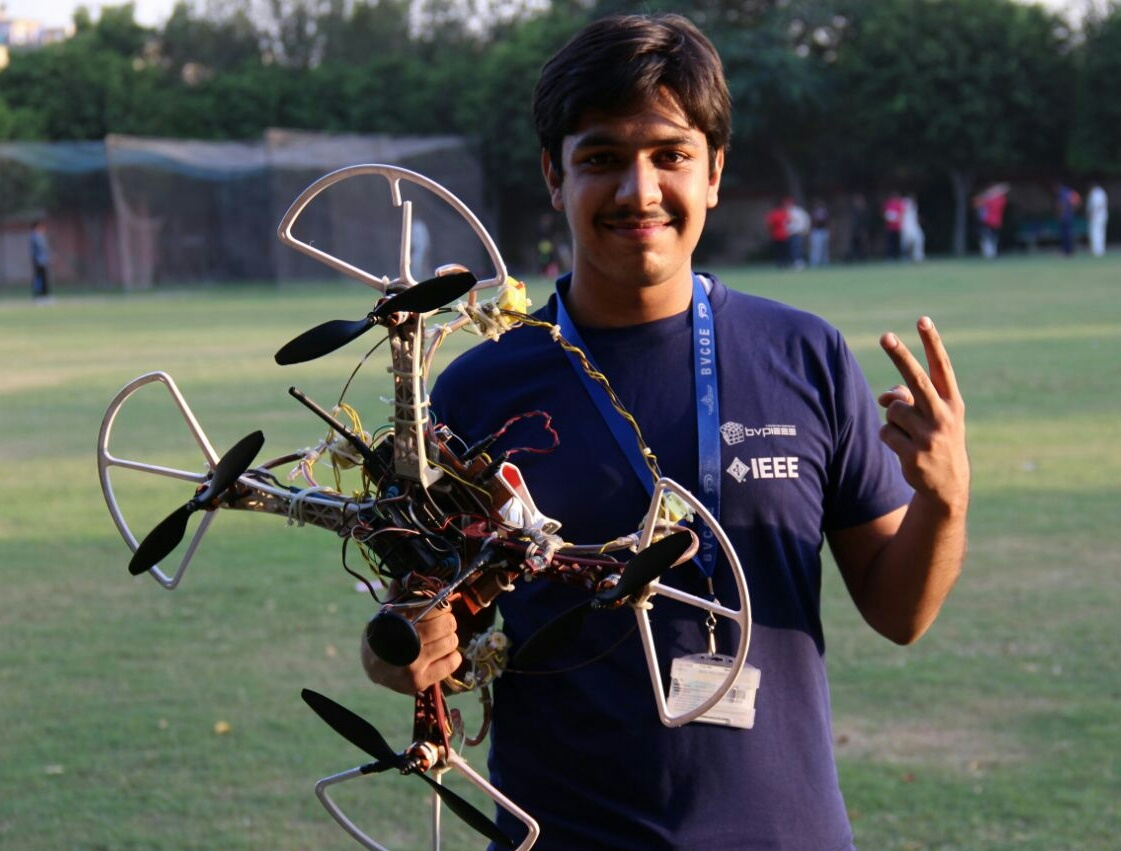
\includegraphics[scale=0.169]{siddhant_image}
\end{center}

\begin{flushleft}
\section{\color{red}Car\color{purple}e\color{black}er Obje\color{purple}ct\color{black}ive}
To secure the rewarding internship at e-Yantra, where I can be mentored by the experts in the field of the embeded system at IIT-Bombay which will be salutary for me to secure a career as a researcher in this field.
	\section{\color{green}Per\color{purple}s\color{black}onal D\color{purple}e\color{black}tai\color{purple}l\color{black}s}
	~
\textbf{Address-}    
    886/2A 
    Preet Vihar, Rohtak.\\
    ~
    Haryana\\
    ~
    124001\\
    ~
    \textbf{Contact}-
    +91 9728466229\\
~
\textbf{E-mail-} \href{mailto:siddhantbhambri@gmail.com}{siddhantbhambri@gmail.com}\\
 ~   
    \textbf{LinkedIn-}
    \href{http://www.linkedin.com/in/siddhant-bhambri-27b7a5111}{http://www.linkedin.com/in/siddhant-bhambri-27b7a5111}
\end{flushleft}

\section{\color{yellow}Edu\color{black}cational Qualifications}
\begin{center}
\begin{tabular}{ |m{4cm}| m{4cm}| m{2cm}| m{3cm}| }
\hline
&&&\\
\begin{center}
\textbf{{ Course/Examination }}
\end{center}&\begin{center}\textbf{ Institute/University }\end{center}&\begin{center}\textbf{ Year of passing }\end{center}&\begin{center}\textbf{ Performance }\end{center}\\
\hline
&&&\\
\begin{center}
B.Tech, Electronics and Communication Engineering
\end{center}& \begin{center}
Bharati Vidyapeeth's College Of Engineering
\end{center}&\begin{center}
2019
\end{center}& \begin{center}
71.00 (C) (up to third semester)
\end{center}\\
\hline
\begin{center}
CBSC (SCIENCE-PCM)\\
XIIth
\end{center}&
\begin{center}
(CBSE) Model School Rohtak, Haryana
\end{center}&
\begin{center}
2015
\end{center}&
\begin{center}
77.00 percent(agg)
\end{center}\\
\hline
\begin{center}
CBSE\\
Xth
\end{center}&
\begin{center}
(CBSE) Model School Rohtak, Haryana
\end{center}&
\begin{center}
2013
\end{center}&
\begin{center}
8.8 CGPA
\end{center}\\
\hline
\end{tabular}
\end{center}
\end{minipage}

\begin{minipage}{1.0\linewidth}

\section{\color{orange}Pro\color{black}jects}
\subsection{Co\color{purple}m\color{black}pl\color{purple}e\color{black}ted}
\begin{enumerate}
\item Model a Terrain using Serial communication between Firebird V and Blender Game Engin using (XBees 2.4C).
\item Interfacing Firebird V, eYRC Labs, IIT Bombay(ATMEGA2560).
\item Autonomous features like auto landing and take-off, Geo-fencing and altitude hold in a multi-copter.
\item Quadcopter system for aerial surveillance using KK2.1.5 board.
\item Bluetooth Controlled Quadcopter Rover Mechanisum using Arduino.
\item IOT based Plug AND Play Home Automation System Without Rewiring. 
\item Making and controlling 8*8*8 multiplexed LED cube matrix with self-built PCB.
\item Tic-tac-toe Game with GUI(Graphic User Interface) in JAVA.
\item RFID, IR sensor,GSM and GPS based anti-car theft system.
\item Propeller Clock  (ATMEGA-8).
\item IoT based Door lock system (TI- CC3200).
\end{enumerate}

\end{minipage}
\end{document}